\pagebreak
\subsection{Manipulación}

A continuación vamos a experimentar que tan manipulable es el algoritmo PageRank a medida que va cambiando el factor de teletransportacion. La idea es la siguiente, un algoritmo con un factor de teletransportacion bajo pondera menos en la matriz de transición el componente de la estructura del grafo. Por lo tanto, un Search Engine que tenga este factor de teletransportacion bajo va a ser sumamente manipulable, dado que puedo crear muchisimos nodos e inflar el ranking de cualquier sitio. Cuanto mayor es este factor, conjeturamos que vamos a observar que inflar cualquier sitio sera mucho mas costoso en termino de cantidad de sitios únicos que debo crear. De hecho, Page \& Brin en su paper consideran esto y mencionan que en Google se ponderan muchos factores para evitar lo que hoy se conoce como SEO (Search Engine Optimization).

Primero vamos a ver las posiblidadades de manipulacion con c = 0.85. Para hacer esto se fijo el valor de c, se tomo una red de 30 nodos y 30 ejes, y a la primer pagina se le agrego una pagina que la apunte por cada iteracion, este proceso se repitio hasta agregar 80 enlaces a la primer pagina. El resultado es:

\begin{figure}[H]
\centering
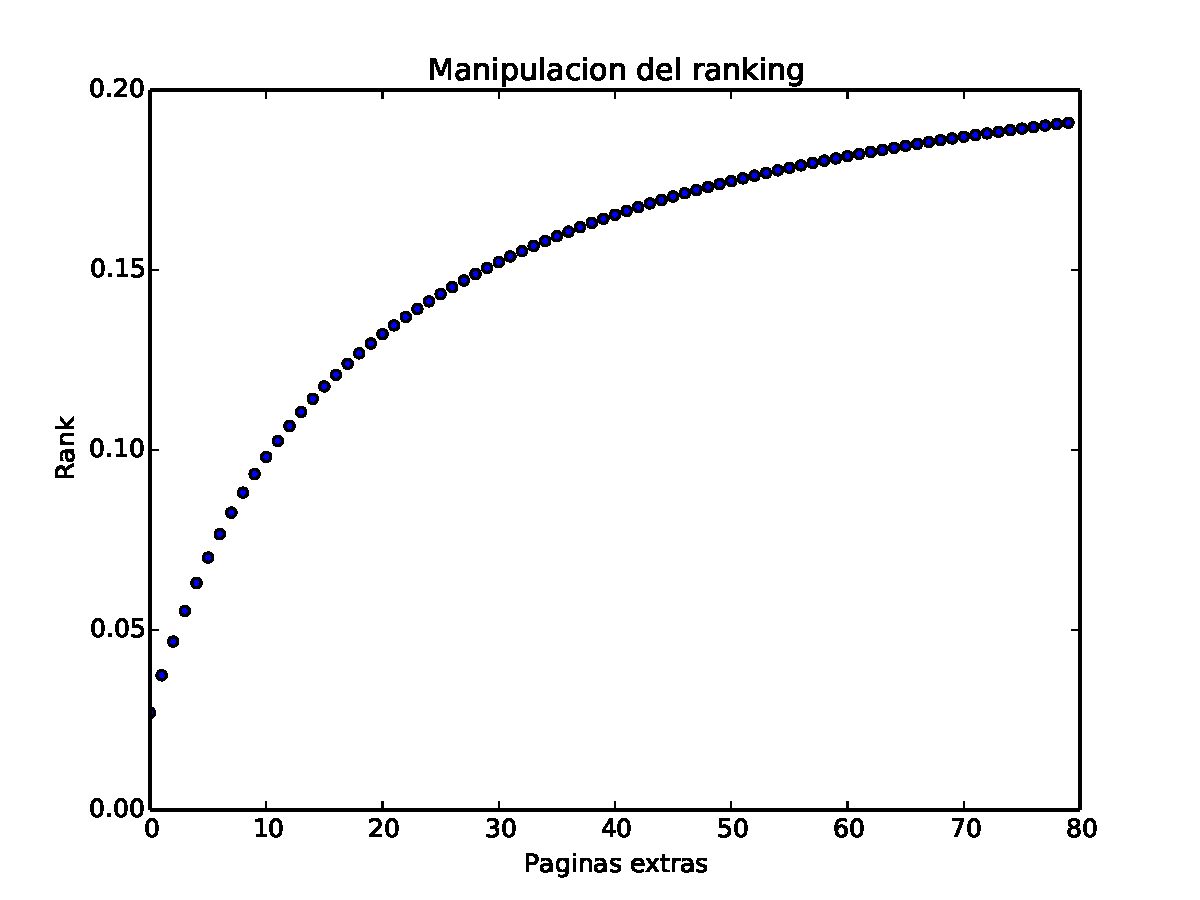
\includegraphics[scale=0.7]{images/manipulacion.pdf}
\caption{A medida que aumenta la cantidad de enlaces, muestra como cambia el ranking.}
\label{timePageRank}
\end{figure}

Como podemos apreciar, la pagina aumenta de posicion en el ranking, pero como podemos apreciar, el beneficio de agregar paginas disminuye con el tiempo.

Para el ultimo caso (es decir, el caso con 80 enlaces extras apuntando a la primer pagina), decidimos ver como influyen los valores de c. Se tomo c = 0, se lo aumento en 0.1, hasta llegar a 0.9. El resultado fue el siguiente:

\begin{figure}[H]
\centering
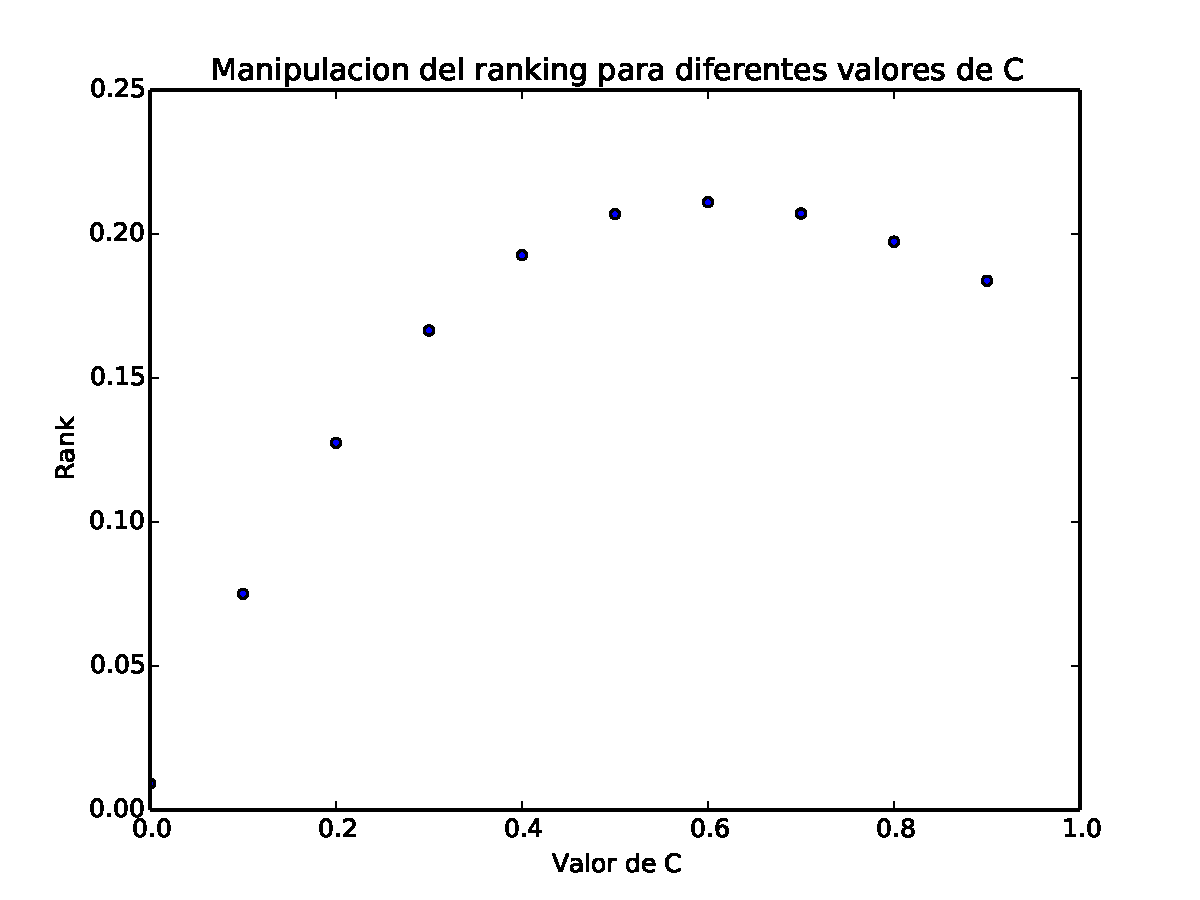
\includegraphics[scale=0.7]{images/manipulacionC.pdf}
\caption{A medida que aumenta la cantidad de enlaces, muestra como cambia el ranking.}
\label{timePageRank}
\end{figure}

En este caso podemos ver como influye el factor de teletranspotacion, si es muy pequeño, la pagina tiene pocas chances de ser visitada mientras que con un valor de 0.6 maximizamos la posiblidad de que sea visitada. Consideramos que la idea no es beneficiar a la manipulacion, pero tampoco se puede elegir un valor que afecte negativamente a paginas con linkeo legitimo, con lo cual podemos ver parte de la motivacion para elegir un valor cerca de 0.6, como puede ser el 0.85 de Page y Brin.
